\documentclass[runningheads]{llncs}
\usepackage[spanish]{babel}
\usepackage{graphicx}
\usepackage{tabularx, booktabs}
\renewcommand{\arraystretch}{1.5}

\begin{document}
\title{GitLab}
\author{David Barragán\inst{1} \and
        Joel Bonilla\inst{1} \and
        Josué García\inst{1} \and
        David Manjarrez\inst{1} \and
        Ariel Paredes Lozada\inst{1}
        }
\institute{Universidad Técnica de Ambato, Ambato, Ecuador\\
\email{secretariageneral@uta.edu.ec}}

\maketitle
\begin{abstract}
        %Abstract de 120 palabras
        El control de versiones, el testeo y monitoreo son una partes fundamentales dentro del desarrollo del software.
        En la actualidad, existen múltiples herramientas que automatizan este proceso, que se engloban bajo el nombre de DevOps.
        Una de estas herramientas de DevOps es GitLab, que facilita el ciclo de desarrollo y facilita la colaboración.
        Es necesario conocer las características, funciones, ventajas y desventajas de esta herramienta con el fin de 
        sopesar su uso y determinar la viabilidad de su uso en proyectos. Por este mismo motivo, es enecesario conocer la
        historia de GitLab, y qué papel juega dentro del panorama de las demás herramientas de DevOps.
        Con este fin, se ha hecho una investigación para determinar las características más importantes de GitLab y
        sintetizarlo en un informe. 
\end{abstract}
\keywords{GitLab \and DevOps \and funciones}
\section{Introducción}
%Qué es el sistema de control de versiones y así
%Panorama para usar GitLab
El desarrollo de software es una tarea colaborativa, con múltiples desarrolladores trabajando juntos en
un mismo proyecto. Sin embargo, manejar un proyecto así es difícil \cite{fairbanks2023analyzing}. Existen
muchos problemas que pueden aparecer en desarrollo, relacionados al manejo de los cambios por parte de los
desarrolladores, a las pruebas continuas en el código y a la integración con las distintas partes.\\
Con el fin de resolver estos problemas, se han propuesto el uso de herramientas que faciliten la colaboración
y monitoreo dentro del desarrollo de software. Este conjunto de herramientas y prácticas que buscan facilitar
y automatizar los procesos de desarrollo de software se denominan DevOps \cite{gitlab2022gitlab}.\\
\begin{figure}[htbp]
        \centering
        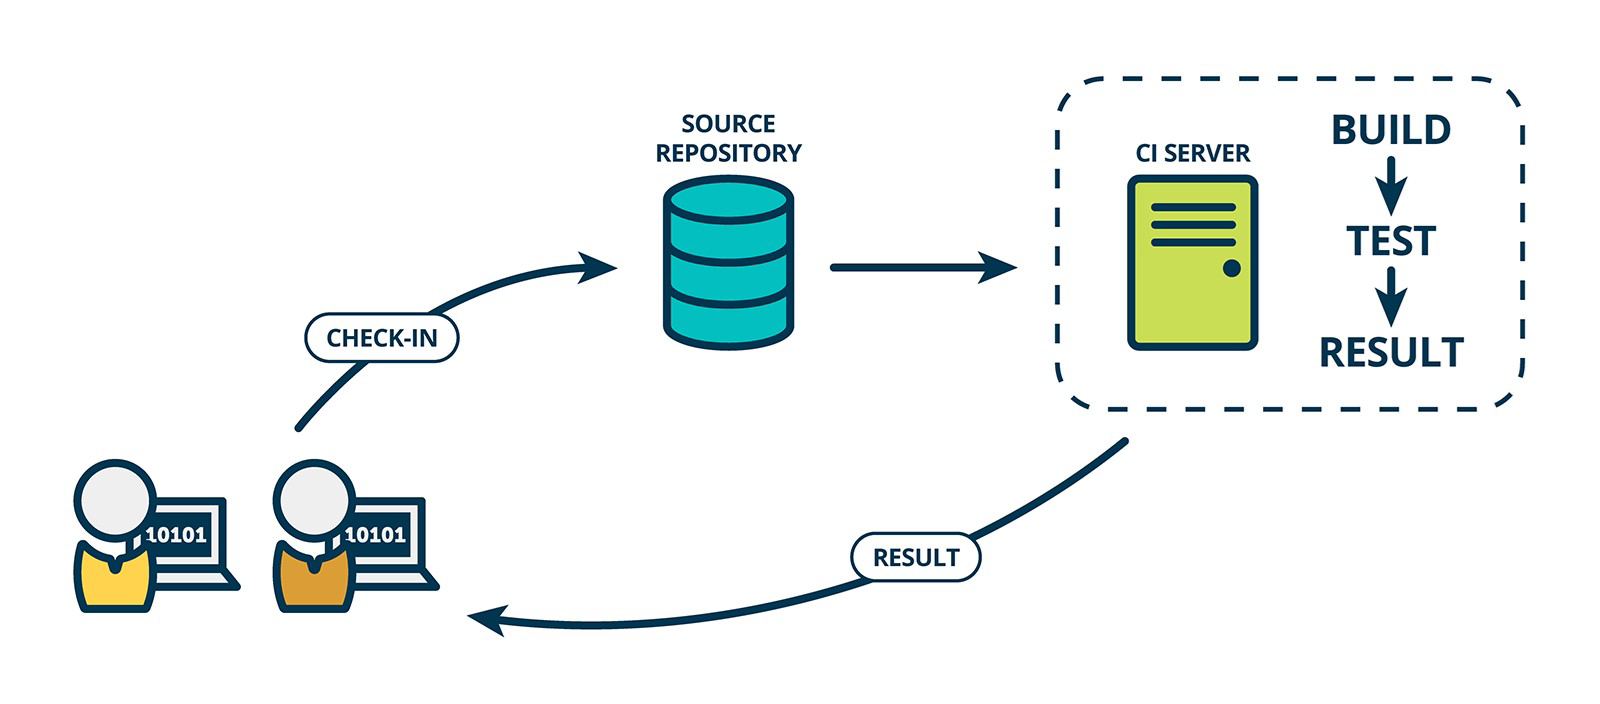
\includegraphics[width=0.5\textwidth]{Dev-Ops.png}
        \caption{Proceso DevOps}
        \label{fig:devops}
\end{figure}
Una de las herramientas de DevOps más conocidas es GitLab, que permite automatizar el ciclo de desarrollo,
desde la planificación y creación hasta las pruebas y el monitoreo de aplicaciones. GitLab es una plataforma
de gestión de repositorios que permite la colaboración entre desarrolladores, así como la automatización de
pruebas y el despliegue del software \cite{safari2020analysis}. GitLab es similar a GitHub, en el sentido de que
ofrece la gestión de repositorios y permite el control de versiones por distintas partes, pero difiere en
que provee de más servicios, enfocados en la integración y entrega continuas (CI/CD, por sus siglas en inglés) \cite{safari2020analysis}.\\
Con el fin de saber más acerca de GitLab y sus aplicaciones, se ha realizado una investigación en
distintas fuentes. Se busca entender las características, ventajas y desventajas de GitLab, con el fin
de explicar las motivaciones de su uso dentro de un proyecto de software. Así mismo, se busa reconocer el
lugar en donde se encuentra GitLab dentro de las herramientas DevOps, mediante una comparación frente a las demás
opciones existentes en el mercado.
\section{Metodología}
%Qué artículos se investigaron
%Bajo qué criterios se escogieron
%De dónde se lo sacó
Se investigó una serie de artículos relacionados al uso de GitLab en distintos proyectos, con el fin
de analizar su uso en el desarrollo de software. En total, se investigaron cinco artículos de fuentes confiables.
Entre estas fuentes se encuentran: Google Scholar y la página web Academia.\\
Los criterios de búsqueda que se usaron para los artículos fueron:
\begin{itemize}
        \item Tener los términos clave "GitLab" y "development", "characteristics" o "DevOps"
        \item Estar publicado desde el 2020 hasta la actualidad
        \item Estar publicado por una institución oficial
        \item De preferencia, que sea una investigación publicada en inglés
\end{itemize}
Se obtuvieron ocho artículos bajo este enfoque. Con el fin de extraer la mayor cantidad de datos de
esta investigación, se siguen la metodología de Revisión Sitemática de la Literatura, con un enfoque
cualitativo.
\subsection{Preguntas de investigación}
%Pon en taxonomía de Bloom
%¿Qué es GitLab?->Objetivo: Identificar qué es GitLab y sus características importantes
%¿Cuáles son las funciones de GitLab?->Objetivo: Qué hace GitLab, sus casos de uso y ejemplos de cosas que usan GitLab
%¿Cuál es la historia de GitLab?->Objetivo: Poner en perspectiva a GitLab en la historia y frente a otros VCSs
%¿Cuáles son las ventajas y desventajas de GitLab?-> Objetivo: Sopesar los pro y contras de GitLab para determinar su uso en proyectos
Se buscan responder cuatro interrogantes con la investigación:
\begin{itemize}
        \item \textbf{RQ1}: ¿Qué es GitLab?\\
        \textit{RQ1-Objetivo}: Identificar las características principales de GitLab, como tipo de licencia y curva de aprendizaje
        \item \textbf{RQ2}: ¿Cuáles son las funciones de GitLab?\\
        \textit{RQ2-Objetivo}: Describir las principales funciones, casos de uso y ejemplos de aplicaciones hechas con GitLab
        \item \textbf{RQ3}: ¿Cuál es la historia de GitLab?\\
        \textit{RQ3-Objetivo}: Compilar el desarrollo de GitLab a lo largo del tiempo y contrastarlo con otras herramientas similares
        \item \textbf{RQ4}: ¿Cuáles son las ventajas y desventajas de GitLab?\\
        \textit{RQ4-Objetivo}: Examinar los pros y contras del desarrollo con GitLab frente a otras herramientas DevOps y enfoques de desarrollo
\end{itemize}
\subsection{Exploración de documentos}
%Se hizo una búsqueda en tal y tal sitios web.
%Se sacaron los artículostal y cual de Google Scholar, los demás de este otro sitio
Se hizo una búsqueda en los sitios web de Google Scholar, Academia, IEEE Xplore, Research Gate e incluso PubMed Central.
Se encontraron los siguientes artículos.
%PD: Pon más artículos si encuentras
\begin{table}[ht!]
        \centering
        \begin{tabular}{l | c | l}
                Base de Datos & Número de artículos consultados & URL \\
                \hline
                \hline
                IEEE Xplorer & 3 & https://ieeexplore.ieee.org/ \\
                Research Gate & 3 & https://www.researchgate.net/ \\
                PubMed & 1 & https://pubmed.ncbi.nlm.nih.gov/ \\
                Google Scholar & 1 & https://scholar.google.com/ 
        \end{tabular}
        \caption{Bases de datos consultadas}
        \label{table:1}
\end{table}
\subsection{Selección de obras}
%Criterios de selección
%Obras desde el 2020, con relación a GitLab
Se encontraron una serie de artículos que hacen referencia a GitLab y a herramientas DevOps. En total se
recuperaron 5 artículos que hacen directa referencia a GitLab, y que proveen información acerca de otras
herramientas de desarrollo.\\
Los artículos se basaron en los siguientes criterios:
\begin{itemize}
        \item Tener los términos clave "GitLab", "development", "characteristics" o "DevOps"
        \item Estar publicado desde el 2020 hasta la actualidad
        \item Estar publicado por una institución oficial
        \item De preferencia, que sea una investigación publicada en inglés
\end{itemize}
Todos los artículos encontrados caen dentro de estos criterios de selección.
%\subsection{Adquisición de datos significativos}
%Resumen breve de las obras, características importantes
\section{Resultados}
\subsection{RQ1: ¿Qué es GitLab?}
%Eso po
GitLab es una herramienta web para DevOps \cite{gitlab2022gitlab}. Es una plataforma web que, además de ofrecer
servicios de gestión de repositorios, provee servicios de integración y entrega continua (CI/CD) \cite{fairbanks2023analyzing}.
GitLab da alojamiento a código, de la misma manera que lo hacen otras plataformas como GitHub, BitBucket, Source-Forge
y LaunchPad \cite{safari2020structural}. Sin embargo, GitLab se diferencia de estas principalmente en que GitLab ofrece más
herramientas para el ciclo de vida del software, incluyendo la ya mencionada CI/CD, la gestión de proyectos e incluye
herramientas como wikis de proyecto y seguimiento de problemas, lo que facilita el desarrollo y el manejo de la gestión
en gran medida \cite{safari2020structural}. Además, GitLab tiene un enfoque en la privacidad y el control del código, ya que
permite a las organizaciones autoalojar sus recursos y no depender de servidores externos. También se debe tomar en cuenta que
GitLab permite la colaboración no sólo entre desarrolladores, sino también con otros roles, como diseñadores y
gerentes de proyecto \cite{choudhury2020gitlab}. Esto permite una mejor colaboración entre las partes relacionadas al
desarrollo de un proyecto.\\
Otra de las características fundamentales de GitLab es que es un proyecto de código abierto, lo que permite a los usuarios
modificar el código fuente de la plataforma. Esto ofrece una gran flexibilidad a la hora de personalizarlo, lo que contrasta
con plataformas similares, que son propiedad de una empresa, como es el caso de GitHub \cite{safari2020structural}. También es
necesario tener en cuenta que GitLab, aunque se pensó inicialmente como una plataforma enfocada a la gestión y manejo del software,
puede ser usada para otra gran cantidad de proyectos. El modelo de trabajo de GitLab, enfocado en la colaboración remota y asincrónica,
la transparencia y la gestión de procesos, permite que muchas otras empresas puedan usar GitLab para implementar modelos de
trabajo remoto \cite{choudhury2020gitlab}.\\
GitLab tiene las siguientes características más relevantes:
\begin{enumerate}
        \item \textit{Año de creación}: 2011
        \item \textit{Licencia}: MIT para la versión gratis, licencia propietaria para la pagada
        \item \textit{Empresa propietaria}: GitLab Inc.
        \item \textit{Lenguaje de implementación}: Ruby, con Ruby on Rails
\end{enumerate}
Existe una gran cantidad de proyectos que usan GitLab, pertenecientes no sólo a empresas propietarias
sino que también lo usan proyectos independientes que integren a programadores de distintas zonas
geográficas \cite{safari2020structural}. Desde hace algún tiempo, varios equipos han comenzado a usar GitLab
gracias a sus capacidades en la integración y entrega continua.\\
Sin embargo, GitLab también tiene limitaciones en comparación a plataformas más especializadas, como lo es GitHub
Por ejemplo, GitLab tienen menos capacidad a la hora de visualizar el código, en contraste con GitHub, por ejemplo.
Además, algunas de la comunidad de GitLab es mucho menor que la de otras plataformas, lo que puede dificultar su uso.
Otra característica importante de GitLab es que maneja un flujo de trabajo particular, con estándares propios referentes
a los nombres de la ramas y a cómo se deben unir entre sí \cite{devineni1version}. Este modelo de ramificación, llamado
GitLab Flow, está basado en GitHub flow, y describe 
%TODO: PON EL GITLAB Flow (REF-GITLAB)
\subsection{RQ2: ¿Cuáles son las funciones de GitLab?}
%Funciones de GitLab
GitLab ofrece muchas funciones que facilitan el desarrollo de software y la colaboración entre equipos. Esto lo
logra mediante varias funciones, enfocadas en la integración y entrega continua, la colaboración entre desarrolladores,
el análisis de desempeño, entre otras, relacionadas a la filosofía de DevOps \cite{fairbanks2023analyzing}.\\
Entre las funciones más importantes que ofrece GitLab se encuentran:
\subsubsection{Control de versiones}
GitLab utiliza a Git como sistema de control de versiones \cite{choudhury2020gitlab}. Esto significa que usa un
manejo de versones basado en \textit{commits}, ramas y todas los servicios que Git tiene. Esto también significa que GitLab
se basa en sistema de control de versiones distribuido, en el cual distintos miembros del equipo pueden trabajar
de forma independiente y luego unir sus cambios \cite{alvin2023devops}.
\begin{figure}[htbp]
        \centering
        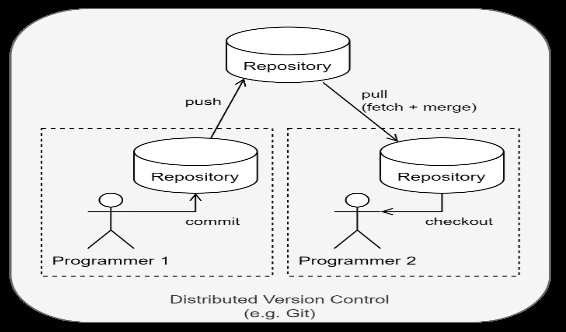
\includegraphics[width=0.5\textwidth]{Distributed.png}
        \caption{Sistema distribuido}
        \label{fig:sys-dis}
\end{figure}
\subsubsection{Alojamiento de código}
Al igual que plataformas como GitHub, GitLab puede alojar código en sus servidores. Sin embargo, en GitHub, el código se almacena
en los servidores de la empresa propietaria. Con GitLab, se pueden usar los servidores de la empresa misma, lo que aumenta la
privacidad. Además, al tener control total sobre los servidores, se pueden gestiónar los proyectos con mucha más libertad y de manera
más personalizada \cite{safari2020structural}.\\
También se pueden gestiónar aspectos de seguridad, ya que se pueden implementar políticas propias de seguridad más estrictas. Este es
el caso de organizaciones que manejen datos sensibles. En sintonía con esto, la empresa puede escalar su infraestructura en caso de
necesitar alojar más datos, o si se necesitan más recursos en general. O, si lo necesita, puede personalizar su instancia de GitLab para
adaptarse a sus flujos de trabajo y procesos específicos.\\
A pesar de todo esto, uno de los problemas obvios con el autoalojamiento es la necesidad de infraestructura, como servidores y máquinas
en general. También está el precio del software, ya que, aunque es posible autoalojar el código con la versión gratutia (la Community Edition),
es preferible usar la versión empresarial (Enterprise Edition) para empresas, ya que ofrece soporte premium y más características \cite{safari2020structural}.
\subsubsection{Integración continua}
Esto hace referencia a la práctica de integrar y probar el código constantemente con el fin de evitar el surgiemiento
de bugs y errores en etapas tempranas. Esto se hace mediante un proceso automatizado de pruebas y construcción de artefactos
cada vez que se realiza un \textit{commit} a las ramas de desarrollo \cite{alvin2023devops,uddin2023comparative}. Esto se logra
mediante un script especializado, que se ejecuta al momento de enviar cambios al repositorio remoto.\\
En el caso de GitLab, este script se lo guarda en el archivo \texttt{.gitlab-ci.yml}. Para las pruebas, se usa el software
de GitLab Runner, el cual se puede personalizar según las necesidades de los desarrolladores.
\subsubsection{Entrega continua}
Es una función referente a la práctica de mantener el código en un estado que esté siempre listo para ser desplegado
en producción \cite{fairbanks2023analyzing}. Lo que se busca es que la aplicación esté lista para llevarse a su entorno
de despliegue.\\
Existen al menos tres entornos de despliegue: de \textit{desarrollo}, de \textit{pruebas} y de \textit{producción}.
Estos entornos se pueden gestiónar mediante ramas en el desarrollo y con contenedores, que empaquetan las aplicaciones
y sus dependencias \cite{fairbanks2023analyzing}. De forma más detallada, se utilizan tres ramas para
gestiónar los entornos.
\begin{table}
        \centering
        \caption{Ramas y entornos de desarrollo}
        \label{table:2}
        \begin{tabularx}{0.9\textwidth}{X | X | X | X}
                \textbf{Entorno de despliegue} & \textbf{Rama de trabajo}
                & \textbf{Rama de origen} & \textbf{Responsable de gestión}\\
                \hline
                Desarrollo & master/main & - & - \\
                Pruebas & testing & master/main & Asesor de calidad \\
                Producción & production & testing & Administrador del sistema\\
                \hline
        \end{tabularx}
\end{table}
Se sigue un flujo de trabajo particular, en el cual cada rama se origina tras hacer un \textit{merge request}
de su rama padre con su rama correspondiente \cite{alvin2023devops}. Se pueden usar tecnologías como Docker 
o máquinas virtuales para implementar los contenedores y guardar el entorno de despliegue de las aplicaciones.
\subsubsection{Colaboración asincrónica}
GitLab permite la colaboración entre miembros de un equipo. Sin embargo, esta puede ser mucho más flexible de lo que sería
una colaboración presencial común y corriente. La colaboración con GitLab puede ser asincrónica y remota, lo que significa
que los miembros del equipo pueden trabajar en sus problemas individuales con comunicación directa mínima, y aun así generar
un buen producto.\\
En GitLab, así como en otros sistemas de control de versiones distribuidos, es posible el desarrollo conjunto mediante ramas
individuales. La integración se hace, justamente, cuando una de estas ramas se una con el flujo principal de desarrollo. Para
nombrar las ramas y gestiónarlas, se sigue el flujo de trabajo de GitLab flow, descrito con anterioridad.\\
El flujo de trabajo, correctamente implementado, es de gran ayuda a la hora de manejar el trabajo conjunto de un equipo.
También es necesario tomar a consideración que, en el contexto actual el trabajo remoto es más común, y el uso de herramientas
como GitLab pueden suponer una gran ventaja a la hora de desarrollar proyectos mediante una modalidad remota \cite{choudhury2020gitlab}
\subsubsection{Planificación de proyectos}
Es necesaria una buena planificación de los proyectos para su éxito. GitLab ofrece herramientas, como tableros Kanban
para visualizar el flujo de trabajo y estado de tareas, la creación de hitos para agrupar \textit{issues} alrededor de
objetivos espeçificos o fechas de entrega, y herramientas de \textit{roadmap} prar visualizar el progreso de los proyectos
a largo plazo \cite{choudhury2020gitlab}.
\subsubsection{Gestión de tareas}
Es necesario organizar el trabajo dentro de cualquier proyecto. GitLab ofrece un manera de crear \textlatin{issues}
para gestiónar tareas específicas. Estos \textit{issues} pueden asignarse a miembros específicos del equipo, pueden
etiquetarse y comentarse con información relevante.\\
Igualmente, dentro de cda \textit{issue} se puede crear una lista de tareas para descomponer el trabajo en trozos más
manejables para un miembro. Esto también facilita el seguimiento del proyecto, para evaluar el nivel de avance en el
proyecto \cite{choudhury2020gitlab}.
\subsubsection{Seguimiento de problemas}
Los errores y problemas sempre aparecen en cualquier proyecto. Para que no lo consuman, es necesario gestiónarlos de
buena manera antes de que se salgan de control. En GitLab, es posible dar un seguimiento a los problemas, reportar
errores, y plantear preguntas \cite{choudhury2020gitlab}.\\
Además, hay que tener en cuenta que los procesos de CD/CI permiten reducir el número de errores que surgan, ya que los
errores se encuentran más rápidamente. Sin embargo, no todo son ventajas, ya que el mismo proceso de CD/CI aumenta la
velocidad a la que se hacen \textit{commit}, pero al mismo tiempo aumenta la cantidad de errores que se introducen en el
código \cite{fairbanks2023analyzing}. Los equipos deben equilibrar este aspecto al usar GitLab.
\subsubsection{Generación de documentación}
La generación de documentación es parte fundamental en el desarrollo de software. Sin embargo, es también una parte muy
tediosa, y suele ser evitada por desarrolladores. Aunque GitLab no ofrece un servicio automatizado para la generación de
documentación, sí posee herramientas que lo facilitan.\\
Entre estas, se encuentra GitLab Pages, que permite crear y publicar sitios web estátitcos directamente desde los repositorios
de GitLab. Esto puede usarse para documentar proyectos o generar wikis que puedan ser usados en el futuro para comprender de
mejor manera el proyecto. Las wikis también se pueden hacer de manera colaborativa, lo que aumenta su valor para el 
equipo \cite{choudhury2020gitlab,safari2020analysis}.\\
También se encuentra Markdown, que es capaz de generar documentación que puede versionarse y gestiónarse de igual manera que el
código. Esto facilita la creación de documentos legibles y bien estructurados que, además, siempre estén actualizados
con la versión actual del proyecto. Esta documentación también está disponible para todo el proyecto, lo que aumenta la
legibilidad del código y facilita la colaboración.
\subsubsection{Control de acceso y seguridad}
Una de las funciones de GitLab es controlar el acceso al proyecto. Esto se logra de múltiples maneras \cite{safari2020structural}.
\begin{itemize}
        \item \textbf{Control de Acceso Basado en Roles}: Se pueden definir roles y permisos específicos para los usuarios
        \item \textbf{Autenticación de Dos Factores}: Hace referencia a que se necesitan dos factores para acceder al proyecto
        \item \textbf{Auditorías}: Es posible rastrear las actividades de los usuarios dentro de la plataforma mediante herramientas de auditoría
        \item \textbf{Protección de Ramas}: Se pueden proteger ramas específicas dentro del repositorio, lo que permite que sólo cambios revisados y aprobados lleguen a la rama principal
        \item \textbf{Escaneo de Vulnerabilidades}: Se escanea el código en búsqueda de vulnerabilidades de seguridad, como contraseñaso claves dentro del código
        \item \textbf{Configuración de políticas de Seguridad}: Se pueden aplicar políticas de privacidad a proyectos y grupos
\end{itemize}
\subsubsection{Personalización}
GitLab permite la integración con muchas tecnologías y servicios externos. Es posible extender las capacidades de GitLab mediante herramientas externas,
como lo son sistemas de gestión de proyectos externos, otras herramientas CI/CD, e incluso tecnologías como lo son los contenedores
Justamente se puede integrar a Docker con GitLab, para mantener un entorno de desarrollo más compacto que tenga en cuenta las aplicaciones
externas de las que depende el proyecto.\\
También se puede personalizar mediante al autoalojamiento, o con la personalización de flujos de trabajo, como se explicó anteriormente. Igualmente,
GitLab posee varias características nativas personalizables, y ofrece una API robusta para la integración con herramientas especializadas.
Además, es posible personalizar a GitLab mediante la modificación del código fuente, al menos en su versión CE. Esto es posible ya que GitLab
es de código abierto, por lo que se pueden agregar funcionalidades y personalizar las existentes según las necesidades \cite{safari2020structural}.
\subsection{Historia de GitLab}
%TODO: Historia de GitLab
GitLab tuvo su origen en 2011, por los ucranianos Dmitriy Zaporozhets y Valery Sizov \cite{gitlab2022gitlab}, como un proyecto de código abierto. Fue
producto de la necesidad de una herramienta de gestión de repositorios que facilitara la colaboración en el desarrollo de software \cite{safari2020analysis}.
A lo largo de los años, fue incorporando más funcionalidades, ha evolucionado ampliamente desde sus orígenes.
%Asegurarse de mencionar a BitBucket y otros sistemas similares
\begin{table}
        \centering
        \caption{Comparación de GitLab}
        \begin{tabularx}{1.1\textwidth}{X || X | X | X | X | X | X}
            Herramienta & Curva de aprendizaje & Tipo de licencia & Empresa propietaria & Año de creación & Lenguaje usado & Ejemplos de uso \\
            \hline
            \hline
            GitLab & Moderada, más fácil si se sabe usar Git & MIT License & GitLab Inc. & 2011 & Ruby (framework Ruby on Rails), Javascript, Go & Varios proyectos de múltiples campos\\
            GitHub & Moderada, más fácil si se sabe usar Git & Licencia propietaria & Microsoft & 2008 & Ruby (framework Ruby on Rails) & La inmensa mayoría de proyectos de software\\
            BitBucket & Moderada & Licencia propietaria & Atlassian & 2008 & Python & Atlassian Jira, Puppet, OpenShift\\
            AWS CodeCommit & Moderada & Servicio de pago basado en uso & Amazon Web Services (AWS) & 2015 & Java, Python, entre otros & ECS, proyectos empresariales y de código abierto\\
            Azure DevOps & Moderada a alta & Licencia propietaria & Microsoft & 2018 & TypeScript & Microsoft Teams, Visual Studio Code, .NET Core\\
            Source Froge & Moderada a alta & Licencias de código abierto (GNU, GPL, MIT, etc.) & Slashdot Media Inc. & 1999 & PHP, Perl & FileZila, Audacity, Apache HTTP Server\\
            \hline
        \end{tabularx}
        \label{table:3}
\end{table}
Sin embargo, y a pesar de las distintas plataformas de alojamiento de repositorios, la plataforma más popular, por un muy amplio
márgen es GitHub \cite{uddin2023comparative}.
\begin{figure}[htbp]
        \centering
        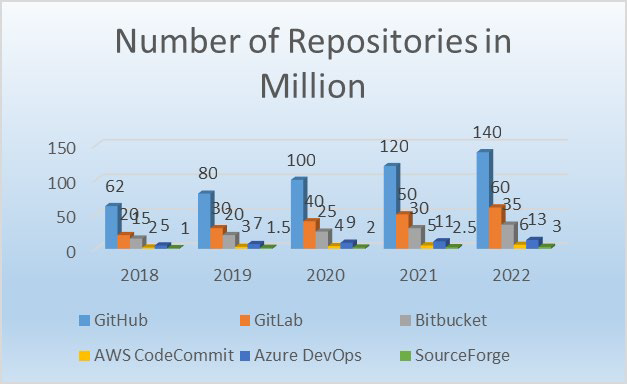
\includegraphics[width=0.5\textwidth]{Comp-rep.png}
        \caption{Comparación entre plataformas}
        \label{fig:comp-rep}
\end{figure}
\subsection{Ventajas y desventajas}
%Ventajas y deventajas de GitLab
%%Una de las desventajas es que aumenta el número de problemas
%Tabla de comparación con otros sistemas similares
\section{Discusión}
%Contextualizar la investigación
%Problemas con la invetigación. Recomendaciones 
\section{Conclusiones}
%Resumen de GitLab, qué hace, para qué se lo usa y qué beneficios tiene
\bibliographystyle{plain}
\bibliography{ref}
\end{document}